\documentclass{article}

% ============================================================================
%  ARCHIVE — Mean queue lengths and mean waiting times
% ----------------------------------------------------------------------------
%  This standalone document preserves the per-model "Mean queue lengths and
%  mean waiting times" subsections that were removed from the main thesis
%  (main.tex) on 2026-06-27.  Each model section below is the verbatim block
%  lifted from its chapter, so nothing is lost.
%
%  NOTE on cross-references: \eqref / \ref / \cite commands that point to
%  objects defined elsewhere in the main thesis (e.g. eq:A:fundamental,
%  thm:A:PGF, cor:A:pi0, the bibliography) are UNDEFINED in this standalone
%  file and will render as "??" / "[?]".  This is expected for an archive;
%  the surrounding derivations are intact.  References internal to a block
%  (e.g. eq:A:Pzz used within the Model-A block) resolve normally.
% ============================================================================

\usepackage[a4paper,top=2cm,bottom=2cm,left=3cm,right=3cm,marginparwidth=1.75cm]{geometry}

\usepackage{amsmath}
\allowdisplaybreaks
\numberwithin{equation}{section}

\usepackage{amsthm}
\usepackage{amssymb}
\usepackage{graphicx}
\usepackage{float}
\usepackage[colorlinks=true, allcolors=blue]{hyperref}
\usepackage{xcolor}
\usepackage{booktabs}
\usepackage{multirow}

\newcommand{\tpi}{\widetilde{\pi}}
\newcommand{\tP}{\widetilde{P}}

% Head-of-line variants (math-mode only).
\newcommand{\BH}{B_2^{\mathrm{H}}}
\newcommand{\CH}{C_2^{\mathrm{H}}}

% Derived numerical macros (\loss*, \uncondWone*, \condWone*, ...) used by the
% loss-fraction section below; same source the main thesis uses.
% Auto-generated by Code/compute_derived_metrics.py -- DO NOT EDIT BY HAND.
% Derived metrics for the Results/Comparison prose. \input this file.

\newcommand{\lossCtwoFifty}{0.166}
\newcommand{\lossCHFifty}{0.156}
\newcommand{\lossCtwoSeventy}{0.232}
\newcommand{\lossCHSeventy}{0.212}
\newcommand{\lossCtwoNinety}{0.297}
\newcommand{\lossCHNinety}{0.266}
\newcommand{\lossCtwoCanon}{0.232}
\newcommand{\lossCHCanon}{0.212}

\newcommand{\lossSysCtwoFifty}{0.071}
\newcommand{\lossSysCHFifty}{0.067}
\newcommand{\lossSysCtwoSeventy}{0.099}
\newcommand{\lossSysCHSeventy}{0.091}
\newcommand{\lossSysCtwoNinety}{0.127}
\newcommand{\lossSysCHNinety}{0.114}
\newcommand{\lossSysCtwoCanon}{0.099}

\newcommand{\lossCtwoThetaLow}{0.044}
\newcommand{\lossCtwoThetaHigh}{0.468}

\newcommand{\condWoneA}{0.9944}
\newcommand{\uncondWoneA}{1.0000}
\newcommand{\fracServedA}{1.000}
\newcommand{\condWoneBtwo}{0.4433}
\newcommand{\uncondWoneBtwo}{0.5151}
\newcommand{\fracServedBtwo}{0.742}
\newcommand{\condWoneCtwo}{0.3863}
\newcommand{\uncondWoneCtwo}{0.4639}
\newcommand{\fracServedCtwo}{0.768}
\newcommand{\condWoneCH}{0.4478}
\newcommand{\uncondWoneCH}{0.5303}
\newcommand{\fracServedCH}{0.788}

\newcommand{\alphaStarA}{0.10}
\newcommand{\ratioPeakA}{0.300}
\newcommand{\alphaStarBtwo}{0.10}
\newcommand{\ratioPeakBtwo}{0.188}
\newcommand{\alphaStarCtwo}{0.90}
\newcommand{\ratioPeakCtwo}{0.357}
\newcommand{\alphaStarBH}{0.10}
\newcommand{\ratioPeakBH}{0.193}
\newcommand{\alphaStarCH}{0.90}
\newcommand{\ratioPeakCH}{0.395}

\newcommand{\ENoneBtwoFifty}{0.0767}
\newcommand{\ENoneBHFifty}{0.0833}
\newcommand{\gapENoneFifty}{0.0067}
\newcommand{\ENoneBtwoSeventy}{0.1545}
\newcommand{\ENoneBHSeventy}{0.1750}
\newcommand{\gapENoneSeventy}{0.0205}
\newcommand{\ENoneBtwoNinety}{0.2626}
\newcommand{\ENoneBHNinety}{0.3115}
\newcommand{\gapENoneNinety}{0.0489}

\newcommand{\PNGetwoAFifty}{0.0230}
\newcommand{\PNGetwoBtwoFifty}{0.0072}
\newcommand{\PNGetwoCtwoFifty}{0.0067}
\newcommand{\PNGetwoBHFifty}{0.0102}
\newcommand{\PNGetwoCHFifty}{0.0095}
\newcommand{\PNGetwoASeventy}{0.0630}
\newcommand{\PNGetwoBtwoSeventy}{0.0193}
\newcommand{\PNGetwoCtwoSeventy}{0.0174}
\newcommand{\PNGetwoBHSeventy}{0.0280}
\newcommand{\PNGetwoCHSeventy}{0.0255}
\newcommand{\PNGetwoANinety}{0.1339}
\newcommand{\PNGetwoBtwoNinety}{0.0399}
\newcommand{\PNGetwoCtwoNinety}{0.0348}
\newcommand{\PNGetwoBHNinety}{0.0595}
\newcommand{\PNGetwoCHNinety}{0.0527}

\newcommand{\premiumASeventy}{3.33}
\newcommand{\premiumBtwoSeventy}{7.18}
\newcommand{\premiumCtwoSeventy}{3.75}
\newcommand{\premiumANinety}{10.00}
\newcommand{\premiumBtwoNinety}{22.38}
\newcommand{\premiumCtwoNinety}{6.30}

\newcommand{\offeredFifty}{0.50}
\newcommand{\throughputAFifty}{0.5000}
\newcommand{\throughputBtwoFifty}{0.5000}
\newcommand{\throughputBHFifty}{0.5000}
\newcommand{\throughputCtwoFifty}{0.4644}
\newcommand{\throughputCHFifty}{0.4667}
\newcommand{\lostflowCtwoFifty}{0.0356}
\newcommand{\lostflowCHFifty}{0.0333}
\newcommand{\offeredSeventy}{0.70}
\newcommand{\throughputASeventy}{0.7000}
\newcommand{\throughputBtwoSeventy}{0.7000}
\newcommand{\throughputBHSeventy}{0.7000}
\newcommand{\throughputCtwoSeventy}{0.6304}
\newcommand{\throughputCHSeventy}{0.6364}
\newcommand{\lostflowCtwoSeventy}{0.0696}
\newcommand{\lostflowCHSeventy}{0.0636}
\newcommand{\offeredNinety}{0.90}
\newcommand{\throughputANinety}{0.9000}
\newcommand{\throughputBtwoNinety}{0.9000}
\newcommand{\throughputBHNinety}{0.9000}
\newcommand{\throughputCtwoNinety}{0.7854}
\newcommand{\throughputCHNinety}{0.7975}
\newcommand{\lostflowCtwoNinety}{0.1146}
\newcommand{\lostflowCHNinety}{0.1025}

\newcommand{\piZeroAFifty}{0.5000}
\newcommand{\piZZAFifty}{0.2500}
\newcommand{\ENAFifty}{0.5000}
\newcommand{\ENtwoAFifty}{0.3636}
\newcommand{\EWoneAFifty}{0.6364}
\newcommand{\EWtwoAFifty}{1.2727}
\newcommand{\piZeroBtwoFifty}{0.5000}
\newcommand{\piZZBtwoFifty}{0.2500}
\newcommand{\ENBtwoFifty}{0.5000}
\newcommand{\ENtwoBtwoFifty}{0.4233}
\newcommand{\EWoneBtwoFifty}{0.3578}
\newcommand{\EWtwoBtwoFifty}{1.4817}
\newcommand{\piZeroCtwoFifty}{0.5356}
\newcommand{\piZZCtwoFifty}{0.2678}
\newcommand{\ENCtwoFifty}{0.3233}
\newcommand{\ENtwoCtwoFifty}{0.2521}
\newcommand{\EWoneCtwoFifty}{0.3323}
\newcommand{\EWtwoCtwoFifty}{0.8823}
\newcommand{\piZeroBHFifty}{0.5000}
\newcommand{\piZZBHFifty}{0.2500}
\newcommand{\ENBHFifty}{0.5000}
\newcommand{\ENtwoBHFifty}{0.4167}
\newcommand{\EWoneBHFifty}{0.3889}
\newcommand{\EWtwoBHFifty}{1.4583}
\newcommand{\piZeroCHFifty}{0.5333}
\newcommand{\piZZCHFifty}{0.2667}
\newcommand{\ENCHFifty}{0.3370}
\newcommand{\ENtwoCHFifty}{0.2593}
\newcommand{\EWoneCHFifty}{0.3630}
\newcommand{\EWtwoCHFifty}{0.9074}
\newcommand{\ENoneAFifty}{0.1364}
\newcommand{\ENoneCtwoFifty}{0.0712}
\newcommand{\ENoneCHFifty}{0.0778}
\newcommand{\piZeroASeventy}{0.3000}
\newcommand{\piZZASeventy}{0.2100}
\newcommand{\ENASeventy}{1.6333}
\newcommand{\ENtwoASeventy}{1.3333}
\newcommand{\EWoneASeventy}{1.0000}
\newcommand{\EWtwoASeventy}{3.3333}
\newcommand{\piZeroBtwoSeventy}{0.3000}
\newcommand{\piZZBtwoSeventy}{0.2100}
\newcommand{\ENBtwoSeventy}{1.6333}
\newcommand{\ENtwoBtwoSeventy}{1.4788}
\newcommand{\EWoneBtwoSeventy}{0.5151}
\newcommand{\EWtwoBtwoSeventy}{3.6970}
\newcommand{\piZeroCtwoSeventy}{0.3696}
\newcommand{\piZZCtwoSeventy}{0.2587}
\newcommand{\ENCtwoSeventy}{0.8358}
\newcommand{\ENtwoCtwoSeventy}{0.6967}
\newcommand{\EWoneCtwoSeventy}{0.4639}
\newcommand{\EWtwoCtwoSeventy}{1.7417}
\newcommand{\piZeroBHSeventy}{0.3000}
\newcommand{\piZZBHSeventy}{0.2100}
\newcommand{\ENBHSeventy}{1.6333}
\newcommand{\ENtwoBHSeventy}{1.4583}
\newcommand{\EWoneBHSeventy}{0.5833}
\newcommand{\EWtwoBHSeventy}{3.6458}
\newcommand{\piZeroCHSeventy}{0.3636}
\newcommand{\piZZCHSeventy}{0.2545}
\newcommand{\ENCHSeventy}{0.9015}
\newcommand{\ENtwoCHSeventy}{0.7424}
\newcommand{\EWoneCHSeventy}{0.5303}
\newcommand{\EWtwoCHSeventy}{1.8561}
\newcommand{\ENoneASeventy}{0.3000}
\newcommand{\ENoneCtwoSeventy}{0.1392}
\newcommand{\ENoneCHSeventy}{0.1591}
\newcommand{\piZeroANinety}{0.1000}
\newcommand{\piZZANinety}{0.0900}
\newcommand{\ENANinety}{8.1000}
\newcommand{\ENtwoANinety}{7.5349}
\newcommand{\EWoneANinety}{1.4651}
\newcommand{\EWtwoANinety}{14.6511}
\newcommand{\piZeroBtwoNinety}{0.1000}
\newcommand{\piZZBtwoNinety}{0.0900}
\newcommand{\ENBtwoNinety}{8.1000}
\newcommand{\ENtwoBtwoNinety}{7.8374}
\newcommand{\EWoneBtwoNinety}{0.6808}
\newcommand{\EWtwoBtwoNinety}{15.2394}
\newcommand{\piZeroCtwoNinety}{0.2146}
\newcommand{\piZZCtwoNinety}{0.1931}
\newcommand{\ENCtwoNinety}{2.1537}
\newcommand{\ENtwoCtwoNinety}{1.9245}
\newcommand{\EWoneCtwoNinety}{0.5941}
\newcommand{\EWtwoCtwoNinety}{3.7421}
\newcommand{\piZeroBHNinety}{0.1000}
\newcommand{\piZZBHNinety}{0.0900}
\newcommand{\ENBHNinety}{8.1000}
\newcommand{\ENtwoBHNinety}{7.7884}
\newcommand{\EWoneBHNinety}{0.8077}
\newcommand{\EWtwoBHNinety}{15.1442}
\newcommand{\piZeroCHNinety}{0.2025}
\newcommand{\piZZCHNinety}{0.1823}
\newcommand{\ENCHNinety}{2.4844}
\newcommand{\ENtwoCHNinety}{2.2084}
\newcommand{\EWoneCHNinety}{0.7157}
\newcommand{\EWtwoCHNinety}{4.2941}
\newcommand{\ENoneANinety}{0.5651}
\newcommand{\ENoneCtwoNinety}{0.2292}
\newcommand{\ENoneCHNinety}{0.2760}

\newcommand{\premiumBHSeventy}{6.25}
\newcommand{\premiumCHSeventy}{3.50}
\newcommand{\premiumBHNinety}{18.75}
\newcommand{\premiumCHNinety}{6.00}

\newcommand{\EWtwoBtwoInflationSeventy}{10.9}
\newcommand{\ENoneBtwoReductionSeventy}{48.5}
\newcommand{\ENoneBHReductionSeventy}{41.7}


\title{Archive: Removed Results\\
\large (mean queue lengths, mean waiting times, and loss fractions;\\
removed from the main thesis and preserved verbatim)}
\author{Victor Dominguez Sainz}

\begin{document}
\maketitle
\tableofcontents

\bigskip
\noindent\emph{This file collects material removed from the main thesis to keep
the focus on the generating-function structure: the per-model mean-queue-length
and mean-waiting-time derivations (Sections~1--5), and the loss-fraction /
cost-of-abandonment analysis (Section~6). Everything is reproduced unchanged.
Cross-references to the main document do not resolve in this standalone file.}

\section{Model-$A$ (baseline, $\gamma_1=\gamma_2=0$, $\theta_1=\theta_2=0$)}

\subsection{Mean queue lengths and mean waiting times}

The results for Model-$A$ are well-studied and standard. However, they will here appear in a slightly different way compared to what usually appears on textbooks —e.g. Adan \& Resing~\cite{adan2002queueing}—, since our states are defined with the number of customers in the \emph{queues} with a busy server, as opposed to those in the system. The customer in service thus contributes to all those with a factor of $\rho$ to the standard results we would typically find. 

\subsubsection{Class-1 marginal PGF and mean queue length}

Setting $y=1$ in the fundamental equation~\eqref{eq:A:fundamental} gives
\begin{align*}
    \begin{split}
        \bigl[-\lambda_1(x-1)(x-1/\rho_1)\bigr]\,P(x,1)
        \;=\; \mu(x-1)\,P_y(1).
    \end{split}
\end{align*}
Cancelling the common factor $(x-1)$ for $x\neq1$ and rearranging:
\begin{align*}
    \begin{split}
        P(x,1) \;=\; \frac{\mu\,P_y(1)}{\mu-\lambda_1 x}.
    \end{split}
\end{align*}
The constant $P_y(1)$ is obtained using normalisation for all busy states $P(1,1)=1-\pi_0=\rho$:
\begin{align*}
    \begin{split}
        \rho \;=\; \frac{\mu\,P_y(1)}{\mu-\lambda_1}
        \quad\Longrightarrow\quad
        P_y(1) \;=\; \rho\,(1-\rho_1),
    \end{split}
\end{align*}
so that
\begin{align*}
    \begin{split}
        P(x,1) \;=\; \frac{\rho(1-\rho_1)}{1-\rho_1 x}.
    \end{split}
\end{align*}
Differentiating by the quotient rule and evaluating at $x=1$:
\begin{align}
    \begin{split}
        \mathbb{E}[N_1]
        \;=\; \left.\frac{d}{dx}P(x,1)\right|_{x=1}
        \;=\; \left.\frac{\rho(1-\rho_1)\cdot\rho_1}{(1-\rho_1 x)^2}\right|_{x=1}
        \;=\; \frac{\rho(1-\rho_1)\,\rho_1}{(1-\rho_1)^2}
        \;=\; \frac{\rho\rho_1}{1-\rho_1}.
    \end{split}
    \label{eq:A:EN1}
\end{align}

\subsubsection{Total queue length from the diagonal}

Setting $x=y=z$ in the kernel polynomial $\lambda_1 x^2-(\lambda_1+\lambda_2+\mu)x+\mu$
shows that $x^*(z)=z$ iff $z\in\{1,\,1/\rho\}$; hence $x^*(z)\neq z$ for all
$z\in(0,1)$ with $\rho<1$. Therefore the ratio
$(z-x^*(z))/(x^*(z)-z)=-1$ throughout $(0,1)$, and the formula of
Theorem~\ref{thm:A:PGF} reduces to:
\begin{align*}
    \begin{split}
        P(z,z)
        \;=\; \frac{z(1-z)\,\rho(1-\rho)}{D(z,z)}\cdot(-1).
    \end{split}
\end{align*}
The denominator at $x=y=z$ is
$D(z,z)=(1+\rho)z^2-z-\rho z^3=-\rho z(z-1)(z-1/\rho)$,
so:
\begin{align}
    \begin{split}
        P(z,z)
        &\;=\; \frac{-z(1-z)\,\rho(1-\rho)}{-\rho z(z-1)(z-1/\rho)} \\
        &\;=\; \frac{(1-z)(1-\rho)}{(z-1)(z-1/\rho)}
         \;=\; \frac{-(1-\rho)}{z-1/\rho}
         \;=\; \frac{\rho(1-\rho)}{1-\rho z},
    \end{split}
    \label{eq:A:Pzz}
\end{align}
confirming the diagonal identity of Corollary~\ref{cor:A:pi0}.
Since $\tfrac{d}{dz}P(z,z)\big|_{z=1}
=\tfrac{\partial }{\partial x}P(1,1)+\tfrac{\partial }{\partial y}P(1,1)
=\mathbb{E}[N_1]+\mathbb{E}[N_2]$, differentiating by the quotient rule and
evaluating at $z=1$ gives:
\begin{align*}
    \begin{split}
        \mathbb{E}[N_1]+\mathbb{E}[N_2]
        \;=\; \left.\frac{d}{dz}\,\frac{\rho(1-\rho)}{1-\rho z}\right|_{z=1}
        \;=\; \frac{\rho(1-\rho)\cdot\rho}{(1-\rho z)^2}\bigg|_{z=1}
        \;=\; \frac{\rho^2(1-\rho)}{(1-\rho)^2}
        \;=\; \frac{\rho^2}{1-\rho}.
    \end{split}
\end{align*}
This is the $M/M/1(\lambda,\mu)$ queue-length formula for the combined
system~\cite{adan2002queueing}, as expected: the two classes together behave as a
single $M/M/1$ queue.

\subsubsection{Class-2 mean queue length}
By subtracting the marginal for class-$1$ to the total number of customers, we find the marginal for class-$2$:
\begin{align}
    \begin{split}
        \mathbb{E}[N_2]
        &\;=\; \bigl(\mathbb{E}[N_1]+\mathbb{E}[N_2]\bigr)-\mathbb{E}[N_1]
        \;=\; \frac{\rho^2}{1-\rho} - \frac{\rho\rho_1}{1-\rho_1} \\[4pt]
        &\;=\; \frac{\rho^2(1-\rho_1)-\rho\rho_1(1-\rho)}{(1-\rho)(1-\rho_1)}
        \;=\; \frac{\rho\bigl[\rho(1-\rho_1)-\rho_1(1-\rho)\bigr]}{(1-\rho)(1-\rho_1)} \\[4pt]
        &\;=\; \frac{\rho(\rho-\rho_1)}{(1-\rho)(1-\rho_1)}
        \;=\; \frac{\rho\rho_2}{(1-\rho_1)(1-\rho)}.
    \end{split}
    \label{eq:A:EN2}
\end{align}

\subsubsection{Mean waiting times via Little's Law}

To obtain ther expected waiting times, we can simply apply \emph{Little's Law} \ref{sec:prelim} to each class independently: we then have $\mathbb{E}[N_i]=\lambda_i\,\mathbb{E}[W_i]$ where $\mathbb{E}[W_i]$ is the mean waiting time in the queue, excluding the time in service. Therefore:
\begin{align}
    \begin{split}
        \mathbb{E}[W_1]
        \;=\; \frac{\mathbb{E}[N_1]}{\lambda_1}
        \;=\; \frac{\rho\rho_1}{\lambda_1(1-\rho_1)}
        \;=\; \frac{\rho\cdot(\lambda_1/\mu)}{\lambda_1(1-\rho_1)}
        \;=\; \frac{\rho}{\mu(1-\rho_1)},
    \end{split}
    \label{eq:A:EW1} \\[4pt]
    \begin{split}
        \mathbb{E}[W_2]
        \;=\; \frac{\mathbb{E}[N_2]}{\lambda_2}
        \;=\; \frac{\rho\rho_2}{\lambda_2(1-\rho_1)(1-\rho)}
        \;=\; \frac{\rho\cdot(\lambda_2/\mu)}{\lambda_2(1-\rho_1)(1-\rho)}
        \;=\; \frac{\rho}{\mu(1-\rho_1)(1-\rho)}.
    \end{split}
    \label{eq:A:EW2}
\end{align}
As expected, class-$1$ benefits from the priority discipline, and $\mathbb{E}[W_2]$ carries the additional penalty factor $1/(1-\rho)$ compared to $\mathbb{E}[W_1]$.

\section{Model-$B_2$ (one-way jockeying, $\gamma_1>0$, $\gamma_2=0$)}

\subsection{Mean queue lengths and mean waiting times}

\subsubsection*{Total queue length from the diagonal}

Setting $x=y=z$ in the reduced fundamental equation~\eqref{eq:B2:fundamental}, the
jockeying convection term $\gamma_1 xy(x-y)\partial_xP$ vanishes at $x=y=z$
(factor $(x-y)=0$), as does the boundary term $\mu(x-y)P_y(y)$.  The remaining
balance is identical to Model-$A$'s, so the same diagonal cancellation gives
\[
    P(z,z) = \frac{\rho(1-\rho)}{1-\rho z},
\]
the same formula as~\eqref{eq:A:Pzz}.  Since $P(z,z)=\mathbb{E}[z^{N_1+N_2}]=\mathbb{E}[z^{N}]$
is the PGF of the total in-queue count $N$, the generating-function identity
$\tfrac{d}{dz}P(z,z)\big|_{z=1}=\mathbb{E}[N_1]+\mathbb{E}[N_2]$ holds;
differentiating by the quotient rule and evaluating at $z=1$:
\begin{align*}
    \mathbb{E}[N_1]+\mathbb{E}[N_2]
    &= \left.\frac{d}{dz}\,\frac{\rho(1-\rho)}{1-\rho z}\right|_{z=1}
     = \frac{\rho(1-\rho)\,\rho}{(1-\rho z)^2}\bigg|_{z=1} \\
    &= \frac{\rho^2(1-\rho)}{(1-\rho)^2}
     = \frac{\rho^2}{1-\rho}.
\end{align*}
One-way jockeying does not alter the total mean queue length relative to
Model-$A$, since the diagonal PGF is unchanged.

\subsubsection*{Class-1 mean queue length}

We extract $\mathbb{E}[N_1]=\tfrac{\partial P}{\partial x}\big|_{(1,1)}$ by first
reducing the fundamental equation~\eqref{eq:B2:fundamental} at $y=1$, and then
differentiating the resulting marginal PGF at $x=1$.

\medskip\noindent\textit{Step~1: marginal PGF $P(x,1)$.}\enspace
Evaluating~\eqref{eq:B2:fundamental} at $y=1$, the bracket multiplying $P$ becomes
$(\lambda_1+\mu)x-\mu-\lambda_1 x^2=-\lambda_1(x-1)(x-1/\rho_1)$, the convection
coefficient is $\gamma_1 x(x-1)$, and the right-hand side reduces to $\mu(x-1)P_y(1)$
(the $\pi(0,0)$ term carries the factor $(1-y)=0$). Every term therefore shares the common
factor $(x-1)$; cancelling it leaves the first-order linear ODE in $x$:
\[
    -\lambda_1(x-1/\rho_1)\,P(x,1) + \gamma_1 x\,\frac{d}{dx}P(x,1) = \mu\,P_y(1).
\]
The integrating factor for this ODE is $e^{-\lambda_1 x/\gamma_1}\,x^{\,\mu/\gamma_1}$
(noting $\lambda_1/\rho_1=\mu$), and integrating from $0$ to $x$ (the boundary term
vanishes since $0^{\mu/\gamma_1}=0$):
\[
    P(x,1)\,e^{-\lambda_1 x/\gamma_1}\,x^{\,\mu/\gamma_1}
    = \frac{\mu\,P_y(1)}{\gamma_1}
    \int_0^x e^{-\lambda_1 t/\gamma_1}\,t^{\,\mu/\gamma_1-1}\,dt.
\]
Rearranging and writing $\alpha=\mu/\gamma_1$ and
$\mathcal{H}(x)=\int_0^x e^{-\lambda_1 t/\gamma_1}\,t^{\,\alpha-1}\,dt$:
\[
    P(x,1) = \frac{\mu\,P_y(1)}{\gamma_1}\,e^{\lambda_1 x/\gamma_1}\,x^{-\alpha}\,\mathcal{H}(x).
\]
The constant $P_y(1)$ follows from $P(1,1)=1-\pi_0=\rho$, which gives
$P_y(1)=\rho\gamma_1/\bigl(\mu\,e^{\lambda_1/\gamma_1}\,\mathcal{H}(1)\bigr)$.

\medskip\noindent\textit{Step~2: differentiate $P(x,1)$ at $x=1$.}\enspace
Writing $P(x,1)=C\cdot f(x)\cdot\mathcal{H}(x)$ with $C=\mu P_y(1)/\gamma_1$ and
$f(x)=e^{\lambda_1 x/\gamma_1}\,x^{-\alpha}$, the product rule together with
Leibniz's rule ($d\mathcal{H}/dx = e^{-\lambda_1 x/\gamma_1}\,x^{\alpha-1}$, the integrand
at the upper limit) gives
\[
    \frac{d}{dx}P(x,1)
    = C\Bigl[f'(x)\,\mathcal{H}(x)+f(x)\,e^{-\lambda_1 x/\gamma_1}\,x^{\alpha-1}\Bigr].
\]
The logarithmic derivative $f'(x)/f(x)=\lambda_1/\gamma_1-\alpha/x=(\lambda_1 x-\mu)/(\gamma_1 x)$,
and the second product term simplifies as
$f(x)\,e^{-\lambda_1 x/\gamma_1}x^{\alpha-1}=x^{-1}$, so
\[
    \frac{d}{dx}P(x,1)
    = \frac{\mu\,P_y(1)}{\gamma_1}\left[
        e^{\lambda_1 x/\gamma_1}\,x^{-\alpha}\,\frac{\lambda_1 x-\mu}{\gamma_1 x}\,\mathcal{H}(x)
        + x^{-1}
    \right].
\]

\medskip\noindent\textit{Step~3: evaluate at $x=1$.}\enspace
\begin{align}
    \mathbb{E}[N_1]
    &= \left.\frac{d}{dx}P(x,1)\right|_{x=1} \nonumber\\
    &= \frac{\mu\,P_y(1)}{\gamma_1}\left[
        e^{\lambda_1/\gamma_1}\,\frac{\lambda_1-\mu}{\gamma_1}\,\mathcal{H}(1) + 1
    \right],
    \label{eq:B2:EN1}
\end{align}
where $\mathcal{H}(1)=\int_0^1 e^{-\lambda_1 t/\gamma_1}\,t^{\,\mu/\gamma_1-1}\,dt
=(\gamma_1/\lambda_1)^{\mu/\gamma_1}\,\gamma(\mu/\gamma_1,\,\lambda_1/\gamma_1)$
and $\gamma(\cdot,\cdot)$ is the lower incomplete gamma function.  The
factor $(\lambda_1-\mu)<0$ (since $\rho_1=\lambda_1/\mu<1$), confirming that
$e^{\lambda_1/\gamma_1}(\lambda_1-\mu)\mathcal{H}(1)/\gamma_1 + 1 > 0$.
No elementary simplification of~\eqref{eq:B2:EN1} is known; the expression
is evaluated numerically.  As $\gamma_1\to0^+$ the
Model-$A$ value~\eqref{eq:A:EN1} is recovered.

\subsubsection*{Class-2 mean queue length by subtraction}

\[
    \mathbb{E}[N_2]
    = \bigl(\mathbb{E}[N_1]+\mathbb{E}[N_2]\bigr)-\mathbb{E}[N_1]
    = \frac{\rho^2}{1-\rho}-\mathbb{E}[N_1].
\]
Since jockeying defections reduce the class-1 queue,
$\mathbb{E}[N_1]$ is smaller than the Model-$A$ value $\rho\rho_1/(1-\rho_1)$,
so $\mathbb{E}[N_2]$ correspondingly exceeds the Model-$A$ value.

\subsubsection*{Mean waiting times via Little's Law}

\textbf{Little's Law} applies here without qualification. It is a rate-conservation
identity --- for any subsystem in which customers are neither created nor destroyed
internally, the time-average number present equals the long-run entry rate times the mean
time an entrant spends inside --- and it holds for \emph{any} positive-recurrent system with
finite mean queue length (here ensured by $\rho<1$, which gives
$\mathbb{E}[N_1]\le\mathbb{E}[N]=\rho^2/(1-\rho)<\infty$ and so makes the jockeying rate
$\gamma_1\mathbb{E}[N_1]$ below a genuine finite rate), requiring neither Poisson input nor
independence. In particular it remains valid even
though one-way jockeying has destroyed the per-class Poisson/renewal structure (the very
obstruction that ruled out a probabilistic route in Step~(ii)). We apply it to each queue
(the waiting line, excluding the customer in service), with $\mathbb{E}[W_i]$ understood as
the mean time a customer spends in Queue~$i$ averaged over all customers that enter it ---
an arrival routed directly into service contributing a zero-length visit.

\emph{Class~1.} Every class-1 arrival is counted as an entrant to Queue~1 at rate
$\lambda_1$ (those finding the server idle enter service at once, contributing zero waiting
time), and each leaves Queue~1 either by entering service or by jockeying to Queue~2. Since
no other stream feeds Queue~1, its throughput is exactly $\lambda_1$, and Little's Law gives
\begin{equation}
    \mathbb{E}[W_1] = \frac{\mathbb{E}[N_1]}{\lambda_1}.
    \label{eq:B2:EW}
\end{equation}

\emph{Class~2.} Queue~2 has \emph{two} input streams: the class-2 Poisson arrivals at rate
$\lambda_2$ and the jockeying transfers from Queue~1. Because each of the $N_1$ waiting
class-1 customers jockeys independently at rate $\gamma_1$, the long-run transfer rate is
$\gamma_1\,\mathbb{E}[N_1]$ (a genuine rate by the ergodic theorem, equal to the time
average of the instantaneous jockeying intensity $\gamma_1 N_1$). The throughput of Queue~2
is therefore $\lambda_2+\gamma_1\,\mathbb{E}[N_1]$, and Little's Law reads
$\mathbb{E}[N_2]=\bigl(\lambda_2+\gamma_1\,\mathbb{E}[N_1]\bigr)\,\mathbb{E}[W_2]$, so that
\begin{equation}
    \mathbb{E}[W_2] = \frac{\mathbb{E}[N_2]}{\lambda_2+\gamma_1\,\mathbb{E}[N_1]}.
    \label{eq:B2:EW2}
\end{equation}
Here $\mathbb{E}[W_2]$ is the mean time in the class-2 line averaged over \emph{all} Queue-2
entrants of both streams; a jockeyed customer's Queue-2 clock starts at the transfer
instant, so its total wait is an initial Queue-1 segment (of mean $\mathbb{E}[W_1]$) followed
by this Queue-2 segment. Thus~\eqref{eq:B2:EW2} is the per-Queue-2-entrant residence time,
not the end-to-end delay of a tagged class-2 \emph{arrival}.

The jockeying inflow is what distinguishes~\eqref{eq:B2:EW2} from the single-stream
Models~$A$ and~$C_2$: the naive denominator $\lambda_2$ would undercount the entrants to
Queue~2 and is correct only in the no-jockeying limit. Indeed, as $\gamma_1\to0^{+}$ the
transfer rate $\gamma_1\,\mathbb{E}[N_1]\to0$, so~\eqref{eq:B2:EW2} reduces to
$\mathbb{E}[N_2]/\lambda_2$ and both~\eqref{eq:B2:EW} and~\eqref{eq:B2:EW2} recover the
Model-$A$ values~\eqref{eq:A:EW1}--\eqref{eq:A:EW2}.

\section{Model-$C_2$ (class-1 abandonment, $\theta_1>0$)}

\subsection{Mean queue lengths and mean waiting times}

\subsubsection*{Why the diagonal no longer simplifies}

Setting $x=y=z$ in~\eqref{eq:C2:fundamental}, the derivative term of abandonment $\theta_1 xy(x-1)\,\partial_xP$ survives (the factor $(x-1)|_{x=z}\neq0$ for $z\in(0,1)$), and the diagonal equation reads
\begin{equation}
    \bigl[(\lambda_1{+}\lambda_2{+}\mu)z^2-\mu z-\lambda z^3\bigr]P(z,z)
    + \theta_1 z^2(z-1)\,\frac{\partial P}{\partial x}(z,z)
    \;=\; -\mu z(1-z)\,\pi(0,0).
    \label{eq:C2:diag}
\end{equation}
The contrast with Model-$A$---or any model without abandonment---is instructive: $P(z,z)$ is no longer purely algebraic with closed form $P(z,z)=\pi(0,0)/(1-\rho z)$~\eqref{eq:A:Pzz}, from which the total $\mathbb{E}[N_1]+\mathbb{E}[N_2]$ followed by a single differentiation. Here the surviving derivative term remains as a second unknown, so that route is no longer available; abandonment removes customers and lowers both means relative to models without it.

\subsubsection*{Class-2 mean queue length via \texorpdfstring{$P(1,y)$}{P(1,y)}}

Setting $x=1$ in~\eqref{eq:C2:fundamental} we obtain
\begin{equation*}
    \lambda_2 y(1-y)\,P(1,y) \;=\; \mu(1-y)\bigl[P_y(y)-\pi(0,0)\bigr].
\end{equation*}
Cancelling $(1-y)$ for $y\neq1$ and substituting the known $P_y(y)$~\eqref{eq:C2:Py},
\begin{equation*}
    P(1,y)
    \;=\; \frac{\mu\bigl[P_y(y)-\pi(0,0)\bigr]}{\lambda_2 y}
    \;=\; \frac{\mu\,\pi(0,0)}{\lambda_2}\cdot\frac{1-\widetilde{B}_C(\lambda_2(1-y))}{\widetilde{B}_C(\lambda_2(1-y))-y},
\end{equation*}
the marginal PGF of class-$2$. It is $0/0$ at $y=1$, so set $\varepsilon=1-y\to0$ and use the LST Taylor expansion $\widetilde{B}_C(\lambda_2\varepsilon)=1-\lambda_2\mathbb{E}[B_C]\,\varepsilon+\tfrac{1}{2}\lambda_2^2\mathbb{E}[B_C^2]\,\varepsilon^2+O(\varepsilon^3)$:
\begin{align*}
    1-\widetilde{B}_C(\lambda_2\varepsilon)
    &\;=\; \lambda_2\mathbb{E}[B_C]\,\varepsilon
           -\tfrac{1}{2}\lambda_2^2\mathbb{E}[B_C^2]\,\varepsilon^2+O(\varepsilon^3), \\
    \widetilde{B}_C(\lambda_2\varepsilon)-y
    &\;=\; \bigl(1-\lambda_2\mathbb{E}[B_C]\,\varepsilon+\tfrac{1}{2}\lambda_2^2\mathbb{E}[B_C^2]\,\varepsilon^2\bigr)-(1-\varepsilon)
    \;=\; (1-\lambda_2\mathbb{E}[B_C])\,\varepsilon
           +\tfrac{1}{2}\lambda_2^2\mathbb{E}[B_C^2]\,\varepsilon^2+O(\varepsilon^3).
\end{align*}
Writing $a=\lambda_2\mathbb{E}[B_C]$ and $c=\tfrac{1}{2}\lambda_2^2\mathbb{E}[B_C^2]$,
\begin{equation*}
    P(1,1-\varepsilon)
    \;=\; \frac{\mu\,\pi(0,0)}{\lambda_2}\cdot\frac{a\varepsilon - c\varepsilon^2+O(\varepsilon^3)}{(1-a)\varepsilon+c\varepsilon^2+O(\varepsilon^3)}
    \;=\; \frac{\mu\,\pi(0,0)}{\lambda_2}\cdot\frac{a-c\varepsilon}{(1-a)+c\varepsilon}+O(\varepsilon^2).
\end{equation*}
Differentiating $f(\varepsilon)=(a-c\varepsilon)/((1-a)+c\varepsilon)$ by the quotient rule,
\begin{equation*}
    f'(\varepsilon)
    \;=\; \frac{-c\,\bigl((1-a)+c\varepsilon\bigr)-(a-c\varepsilon)\,c}{\bigl((1-a)+c\varepsilon\bigr)^2}
    \;=\; \frac{-c}{(1-a+c\varepsilon)^2},
\end{equation*}
and since $\tfrac{d}{dy}P(1,y)\big|_{y=1}=-\tfrac{d}{d\varepsilon}P(1,1-\varepsilon)\big|_{\varepsilon=0}$,
\begin{equation}
    \mathbb{E}[N_2]
    \;=\; \frac{d}{dy}P(1,y)\bigg|_{y=1}
    \;=\; \frac{\mu\,\pi(0,0)}{\lambda_2}\cdot\frac{c}{(1-a)^2}
    \;=\; \frac{\mu\,\pi(0,0)\,\lambda_2\,\mathbb{E}[B_C^2]}{2\,(1-\lambda_2\mathbb{E}[B_C])^2}.
    \label{eq:C2:EN2}
\end{equation}
As $\theta_1\to0^+$, $\mathbb{E}[B_C]\to(\mu-\lambda_1)^{-1}$ and $\mathbb{E}[B_C^2]\to2\mu/(\mu-\lambda_1)^3$, recovering the Model-$A$ value $\mathbb{E}[N_2]=\rho\rho_2/((1-\rho_1)(1-\rho))$.

\subsubsection*{Class-1 mean queue length}

We extract $\mathbb{E}[N_1]=\tfrac{\partial P}{\partial x}\big|_{(1,1)}$ by evaluating the theorem formula at $y=1$ and then differentiating in $x$.

\medskip\noindent\textit{Step~1: marginal PGF $P(x,1)$.}\enspace
As $y\to1$, the exponent $\beta(y)\to0$, so $(1-x)^{\beta(y)}\to1$ for fixed $x\in(0,1)$, and $\mathcal{H}_1(x,y)\to\int_0^x e^{-\lambda_1 t/\theta_1}\,t^{\,\mu/\theta_1-1}\,dt$ while $\mathcal{H}_2(x,y)$ tends to a finite limit. In the theorem's bracket the two integrals carry different weights: $\widetilde{B}_C(\lambda_2(1-y))\to1$, while $1-\widetilde{B}_C(\lambda_2(1-y))=\lambda_2\mathbb{E}[B_C]\,(1-y)+O((1-y)^2)\to0$, so the $\mathcal{H}_2$ term drops and the bracket collapses to $\mathcal{H}_1(x,1)$. The prefactor's $y$-dependent part satisfies $(1-y)/(\widetilde{B}_C(\lambda_2(1-y))-y)\to1/(1-\lambda_2\mathbb{E}[B_C])$, so
\begin{equation*}
    P(x,1)
    \;=\; \frac{\mu\,\pi(0,0)}{\theta_1\,(1-\lambda_2\mathbb{E}[B_C])}\,e^{\lambda_1 x/\theta_1}\,x^{-\mu/\theta_1}
    \int_0^x e^{-\lambda_1 t/\theta_1}\,t^{\,\mu/\theta_1-1}\,dt.
\end{equation*}

\medskip\noindent\textit{Step~2: differentiate $P(x,1)$ at $x=1$.}\enspace
Write $P(x,1)=C\,f(x)\,\mathcal{K}(x)$ with $C=\mu\pi(0,0)/(\theta_1(1-\lambda_2\mathbb{E}[B_C]))$, $f(x)=e^{\lambda_1 x/\theta_1}x^{-\mu/\theta_1}$ and $\mathcal{K}(x)=\int_0^x e^{-\lambda_1 t/\theta_1}t^{\,\mu/\theta_1-1}\,dt$. By the product rule with Leibniz's rule ($\mathcal{K}'(x)=e^{-\lambda_1 x/\theta_1}x^{\mu/\theta_1-1}$) and the logarithmic derivative $f'(x)/f(x)=(\lambda_1 x-\mu)/(\theta_1 x)$,
\begin{equation*}
    \frac{d}{dx}P(x,1)
    \;=\; C\Bigl[f'(x)\,\mathcal{K}(x)+f(x)\,e^{-\lambda_1 x/\theta_1}x^{\mu/\theta_1-1}\Bigr]
    \;=\; C\left[e^{\lambda_1 x/\theta_1}x^{-\mu/\theta_1}\,\frac{\lambda_1 x-\mu}{\theta_1 x}\,\mathcal{K}(x) + x^{-1}\right].
\end{equation*}

\medskip\noindent\textit{Step~3: evaluate at $x=1$.}\enspace
\begin{equation*}
    \mathbb{E}[N_1]
    \;=\; \left.\frac{d}{dx}P(x,1)\right|_{x=1}
    \;=\; \frac{\mu\,\pi(0,0)}{\theta_1\,(1-\lambda_2\mathbb{E}[B_C])}
    \left[e^{\lambda_1/\theta_1}\,\frac{\lambda_1-\mu}{\theta_1}\,\mathcal{K}(1) + 1\right],
\end{equation*}
where $\mathcal{K}(1)=\int_0^1 e^{-\lambda_1 t/\theta_1}t^{\,\mu/\theta_1-1}\,dt=(\theta_1/\lambda_1)^{\mu/\theta_1}\,\gamma(\mu/\theta_1,\,\lambda_1/\theta_1)$, with $\gamma(\cdot,\cdot)$ the lower incomplete gamma function. Since $\lambda_1-\mu<0$ ($\rho_1<1$) the bracket is positive. No elementary simplification is known, so $\mathbb{E}[N_1]$ is evaluated numerically; as $\theta_1\to0^+$ it recovers the Model-$A$ value~\eqref{eq:A:EN1}.

\subsubsection*{Mean waiting times via Little's Law}

The relation $\mathbb{E}[N_i]=\lambda_i\,\mathbb{E}[W_i]$ holds for any stable system. Here $\lambda_i$ is the arrival rate of \emph{all} class-$i$ customers, including those that eventually abandon, so $\mathbb{E}[W_i]$ is the mean queueing time averaged over both served and abandoned customers:
\begin{equation*}
    \mathbb{E}[W_1] \;=\; \frac{\mathbb{E}[N_1]}{\lambda_1},
    \qquad
    \mathbb{E}[W_2] \;=\; \frac{\mathbb{E}[N_2]}{\lambda_2}.
\end{equation*}
Using the throughput $\mu(1-\pi_0)$ instead would give the conditional waiting time of served customers only---a different object. As $\theta_1\to0^+$ both means recover the Model-$A$ values~\eqref{eq:A:EN1}--\eqref{eq:A:EW2}.

\section{Model-$\BH$ (head-of-line jockeying)}

\subsection{Mean queue lengths and mean waiting times}

\subsubsection{Class-1 marginal PGF and mean queue length}

Setting $y=1$ in the fundamental equation~\eqref{eq:B21:fundamental}, the term
$\mu x(1-y)\pi(0,0)$ vanishes and the coefficient of $P(x,1)$ factors as
$-(x-1)\bigl(\lambda_1 x-(\mu+\gamma_1)\bigr)$, while the right-hand side becomes
$(x-1)(\mu+\gamma_1)P_y(1)$. Cancelling $(x-1)$ for $x\ne1$,
\begin{equation}
    P(x,1) \;=\; \frac{(\mu+\gamma_1)\,P_y(1)}{\mu+\gamma_1-\lambda_1 x}
            \;=\; \frac{P_y(1)}{1-\rho_B\,x},
    \qquad \rho_B := \frac{\lambda_1}{\mu+\gamma_1}.
    \label{eq:B21:Px1}
\end{equation}
This is a geometric class-$1$ marginal: the priority queue behaves as an $M/M/1$ queue whose
effective \emph{clearance rate} is $\mu+\gamma_1$, since a waiting class-$1$ customer at the
head of Queue~1 departs that queue either by entering service (rate $\mu$) or by jockeying
(rate $\gamma_1$). The constant $P_y(1)$ is pinned by the normalisation
$P(1,1)=1-\pi_0=\rho$, giving $P_y(1)=\rho(1-\rho_B)$, so that
$P(x,1)=\rho(1-\rho_B)/(1-\rho_B x)$. Differentiating by the quotient rule and evaluating at
$x=1$,
\begin{equation}
    \mathbb{E}[N_1] \;=\; \left.\frac{d}{dx}P(x,1)\right|_{x=1}
    \;=\; \frac{\rho(1-\rho_B)\,\rho_B}{(1-\rho_B)^2}
    \;=\; \frac{\rho\,\rho_B}{1-\rho_B}.
    \label{eq:B21:EN1}
\end{equation}
This is Model-$A$'s formula~\eqref{eq:A:EN1} with the priority load $\rho_1$ replaced by the
\emph{jockeying-reduced} load $\rho_B=\lambda_1/(\mu+\gamma_1)\le\rho_1$.

\subsubsection{Total queue length from the diagonal}

Because jockeying conserves the total number of customers, the combined process
$N_1+N_2$ (together with the in-service customer) is the queue-length process of an ordinary
$M/M/1(\lambda,\mu)$ queue, and the diagonal generating
function~\eqref{eq:B21:Pzz} is $P(z,z)=\rho(1-\rho)/(1-\rho z)$. Since
$\tfrac{d}{dz}P(z,z)\big|_{z=1}=\mathbb{E}[N_1]+\mathbb{E}[N_2]$, differentiating gives
\begin{equation}
    \mathbb{E}[N_1]+\mathbb{E}[N_2]
    \;=\; \left.\frac{d}{dz}\,\frac{\rho(1-\rho)}{1-\rho z}\right|_{z=1}
    \;=\; \frac{\rho^2(1-\rho)}{(1-\rho)^2}
    \;=\; \frac{\rho^2}{1-\rho},
    \label{eq:B21:EN}
\end{equation}
identical to the combined $M/M/1$ result of Model-$A$~\eqref{eq:A:EN2}.

\subsubsection{Class-2 mean queue length by subtraction}

Subtracting~\eqref{eq:B21:EN1} from~\eqref{eq:B21:EN},
\begin{equation}
    \mathbb{E}[N_2]
    \;=\; \frac{\rho^2}{1-\rho} - \frac{\rho\,\rho_B}{1-\rho_B}
    \;=\; \frac{\rho\,(\rho-\rho_B)}{(1-\rho)(1-\rho_B)}.
    \label{eq:B21:EN2}
\end{equation}
The excess load admits a transparent decomposition,
\begin{equation*}
    \rho-\rho_B
    = \frac{\lambda_1+\lambda_2}{\mu} - \frac{\lambda_1}{\mu+\gamma_1}
    = \frac{(\lambda_1+\lambda_2)(\mu+\gamma_1)-\lambda_1\mu}{\mu(\mu+\gamma_1)}
    = \frac{\lambda_2\mu+\lambda_1\gamma_1+\lambda_2\gamma_1}{\mu(\mu+\gamma_1)}
    = \rho_2 + \frac{\lambda_1\gamma_1}{\mu(\mu+\gamma_1)},
\end{equation*}
so $\rho-\rho_B$ exceeds the bare class-$2$ load $\rho_2$ precisely by the load that
jockeying transfers from Queue~1 into Queue~2. At $\gamma_1=0$ it collapses to $\rho_2$
and~\eqref{eq:B21:EN2} recovers Model-$A$'s
$\mathbb{E}[N_2]=\rho\rho_2/[(1-\rho_1)(1-\rho)]$.

\subsubsection{Mean waiting times via Little's Law}

We apply \textbf{Little's Law} to each queue separately, recalling that $N_i$ counts only
the customers \emph{waiting}, so $\mathbb{E}[N_i]=\Lambda_i\,\mathbb{E}[W_i]$ with
$\Lambda_i$ the long-run rate at which customers \emph{enter} Queue~$i$ and $\mathbb{E}[W_i]$
their mean residence time in that queue (from entry until they leave it, by service entry or
by jockeying).

Every class-$1$ customer enters Queue~1 exactly once, by exogenous arrival, so
$\Lambda_1=\lambda_1$ and
\begin{equation*}
    \mathbb{E}[W_1] \;=\; \frac{\mathbb{E}[N_1]}{\lambda_1}
    \;=\; \frac{\rho\,\rho_B}{\lambda_1(1-\rho_B)}
    \;=\; \frac{\rho}{\mu+\gamma_1-\lambda_1}.
\end{equation*}
Compared with Model-$A$'s $\mathbb{E}[W_1]=\rho/(\mu-\lambda_1)$~\eqref{eq:A:EW1}, the
denominator is enlarged by $\gamma_1$: head-of-line jockeying drains the priority queue
faster and shortens class-$1$ waits.

Queue~2 receives a \emph{mixed} input: the exogenous Poisson stream at rate $\lambda_2$
together with the jockeying stream. The latter fires at rate $\gamma_1$ whenever $N_1\ge1$,
so its long-run rate is $\gamma_1\,\mathbb{P}(N_1\ge1)$. The probability that a class-$1$
customer is waiting follows from the geometric marginal~\eqref{eq:B21:Px1} by subtracting
the $N_1=0$ mass from the busy mass,
\begin{equation*}
    \mathbb{P}(N_1\ge1) = P(1,1)-P(0,1) = \rho - \rho(1-\rho_B) = \rho\rho_B,
\end{equation*}
since $P(1,1)=1-\pi_0=\rho$ and $P(0,1)=P_y(1)=\rho(1-\rho_B)$. The total entrance rate into
Queue~2 is therefore $\Lambda_2=\lambda_2+\gamma_1\rho\rho_B$, and Little's Law gives the
mean residence time per Queue-2 entrant,
\begin{equation}
    \mathbb{E}[W_2] \;=\; \frac{\mathbb{E}[N_2]}{\Lambda_2}
    \;=\; \frac{\rho\,(\rho-\rho_B)}
               {(1-\rho)(1-\rho_B)\,\bigl(\lambda_2+\gamma_1\rho\rho_B\bigr)}.
    \label{eq:B21:EW2}
\end{equation}
As $\gamma_1\to0^+$ the jockeying stream disappears, $\Lambda_2\to\lambda_2$ and
$\rho_B\to\rho_1$, and~\eqref{eq:B21:EW2} recovers Model-$A$'s
$\mathbb{E}[W_2]=\rho/[\mu(1-\rho_1)(1-\rho)]$~\eqref{eq:A:EW2}.

\section{Model-$\CH$ (head-of-line abandonment)}

\subsection{Mean queue lengths and mean waiting times}

\subsubsection{Class-1 marginal PGF and mean queue length}

The class-$1$ marginal is the geometric law~\eqref{eq:C21:Px1}; pinning the constant by
$P(1,1)=1-\pi_0$ as in~\eqref{eq:C21:P11} gives $P(x,1)=(1-\pi_0)(1-\rho_C)/(1-\rho_C x)$.
Differentiating and evaluating at $x=1$,
\begin{equation}
    \mathbb{E}[N_1] \;=\; \left.\frac{d}{dx}P(x,1)\right|_{x=1}
    \;=\; \frac{(1-\pi_0)\,\rho_C}{1-\rho_C},
    \qquad \rho_C=\frac{\lambda_1}{\mu+\theta_1},
    \label{eq:C21:EN1}
\end{equation}
with $1-\pi_0=\lambda(\mu+\theta_1)/\bigl[\mu(\mu+\theta_1)+\lambda_1\theta_1\bigr]$ from
Corollary~\ref{cor:C21:pi0}. As in Model-$\BH$, the priority queue behaves as an $M/M/1$
queue with effective clearance rate $\mu+\theta_1$, the only difference from
Model-$\BH$'s~\eqref{eq:B21:EN1} being the prefactor $1-\pi_0$, which here is no longer
equal to $\rho$ because abandonment alters the idle probability.

\subsubsection{Class-2 mean queue length}

Abandonment is a true departure and so breaks the \emph{conservation of the total customer
count} that underlies the diagonal argument: in Model-$\BH$ the jockeying factor
$\gamma_1 y(x-y)$ vanishes on the diagonal $x=y$, whereas here the abandonment factor
$\theta_1 y(x-1)$ does not. Concretely, setting $x=y=z$ in~\eqref{eq:C21:fundamental} leaves
the term $\theta_1 z(z-1)P_y(z)$ on the right-hand side, so the diagonal equation no longer
closes and the route that furnished $\mathbb{E}[N_1]+\mathbb{E}[N_2]$ for Model-$\BH$ is
unavailable. We instead differentiate the class-$2$ marginal. From the
marginal relation~\eqref{eq:C21:P1y}, $P(1,y)=\mu\bigl[P_y(y)-\pi(0,0)\bigr]/(\lambda_2 y)$,
and since $\mathbb{E}[N_2]=\tfrac{d}{dy}P(1,y)\big|_{y=1}$,
\begin{equation}
    \mathbb{E}[N_2]
    \;=\; \frac{\mu}{\lambda_2}\,P_y'(1) - (1-\pi_0),
    \label{eq:C21:EN2_implicit}
\end{equation}
where we used $\tfrac{\mu}{\lambda_2}\bigl[P_y(1)-\pi(0,0)\bigr]=P(1,1)=1-\pi_0$. It remains
to compute $P_y'(1)$ from~\eqref{eq:C21:Py}. Both the numerator $\mu x^*(y)(1-y)\pi(0,0)$ and
the denominator $\Delta(y)=(\mu+\theta_1 y)x^*(y)-y(\mu+\theta_1)$ vanish at $y=1$ (since
$x^*(1)=1$ gives $\Delta(1)=(\mu+\theta_1)-(\mu+\theta_1)=0$), so $P_y(y)$ is a $0/0$ form
there. Writing $N(y)$ and $\Delta(y)$ for numerator and denominator, a second-order Taylor
expansion about $y=1$ gives the value and the slope
\begin{equation*}
    P_y(1) = \frac{N'(1)}{\Delta'(1)} = (1-\pi_0)(1-\rho_C),
    \qquad
    P_y'(1) = \frac{N''(1)\,\Delta'(1) - N'(1)\,\Delta''(1)}{2\,\Delta'(1)^2},
\end{equation*}
which is why both the first and the second root sensitivities of $x^*$ at $y=1$ are needed,
namely~\eqref{eq:C21:xstar_deriv} together with
\begin{equation*}
    \frac{d^2}{dy^2}x^*(1) = \frac{2(\mu+\theta_1)\,\lambda_2^2}{(\mu+\theta_1-\lambda_1)^3}
\end{equation*}
(the latter obtained by differentiating $x^*(y)$ in~\eqref{eq:C21:xstar} twice).
Substituting these into $P_y'(1)$, then into~\eqref{eq:C21:EN2_implicit}, and simplifying
yields the closed form
\begin{equation}
    \mathbb{E}[N_2]
    \;=\; \frac{\lambda_2\,\lambda\,(\mu+\theta_1)\bigl[(\mu+\theta_1)^2-\lambda_1\theta_1\bigr]}
               {(\mu+\theta_1-\lambda_1)\,
                \bigl[\mu(\mu+\theta_1)+\lambda_1\theta_1\bigr]\,
                \bigl[(\mu+\theta_1)(\mu-\lambda)+\lambda_1\theta_1\bigr]},
    \label{eq:C21:EN2}
\end{equation}
with $\lambda=\lambda_1+\lambda_2$. The last bracket in the denominator is exactly the
stability numerator of $\pi_0$ from~\eqref{eq:C21:pi0_pi00}, so $\mathbb{E}[N_2]$ is finite
precisely under the stability condition~\eqref{eq:C21:stability} and diverges as
$\pi_0\to0^+$. As $\theta_1\to0^+$ the right-hand side reduces to
$\lambda_2\lambda/[(\mu-\lambda_1)(\mu-\lambda)]=\rho\rho_2/[(1-\rho_1)(1-\rho)]$, recovering
Model-$A$'s~\eqref{eq:A:EN2}.

\subsubsection{Mean waiting times via Little's Law}

We apply \textbf{Little's Law} to each queue. Every class-$1$ customer enters Queue~1 once
by exogenous arrival and later leaves it either by entering service or by abandoning from the
head; in both cases it leaves Queue~1, so the entrance rate is $\Lambda_1=\lambda_1$ and
\begin{equation*}
    \mathbb{E}[W_1] \;=\; \frac{\mathbb{E}[N_1]}{\lambda_1}
    \;=\; \frac{(1-\pi_0)\,\rho_C}{\lambda_1(1-\rho_C)}.
\end{equation*}
Here $\mathbb{E}[W_1]$ is the mean time a class-$1$ customer spends \emph{waiting} in
Queue~1, averaged over all class-$1$ arrivals, whether they are eventually served or
abandon. Queue~2, by contrast, receives no jockeying input and its customers never abandon
($\theta_2=0$), so every class-$2$ arrival is eventually served and the entrance rate is
simply $\Lambda_2=\lambda_2$:
\begin{equation*}
    \mathbb{E}[W_2] \;=\; \frac{\mathbb{E}[N_2]}{\lambda_2}
\end{equation*}
with $\mathbb{E}[N_2]$ from~\eqref{eq:C21:EN2}, the $\lambda_2$ cancelling against its
numerator. Both means reduce to the corresponding Model-$A$ expressions as $\theta_1\to0^+$.

\section{Loss fractions: the cost of abandonment}

\subsubsection{The cost of abandonment in lost customers}
\label{subsec:comp:abandonment}

The headline gains of $C_2$ --- shorter queues, larger idle fraction, lower priority waiting
time --- are bought with lost customers, and the price is exact in closed form. The server
delivers carried work at rate $\mu(1-\pi_0)$ and the offered rate is $\lambda_1+\lambda_2=\mu\rho$.
Since in steady state every arrival is either served or abandons, flow conservation forces the
total abandonment rate to equal the \emph{idle excess} that abandonment creates over the
no-attrition baseline,
\begin{equation}\label{eq:comp:loss}
  \Lambda_{\mathrm{loss}}
  \;=\;\mu\rho-\mu(1-\pi_0)
  \;=\;\mu\bigl(\pi_0-(1-\rho)\bigr),
\end{equation}
the strictly positive gap $\pi_0-(1-\rho)>0$ of Corollary~\ref{cor:C2:pi00}. The identity
\eqref{eq:comp:loss} holds for either abandonment rate --- the full-rate mechanism realises
$\Lambda_{\mathrm{loss}}=\theta_1\mathbb{E}[N_1]$ and the head-of-line mechanism
$\Lambda_{\mathrm{loss}}=\theta_1\,\mathbb{P}(N_1\ge1)$ --- because it uses only the carried
rate $\mu(1-\pi_0)$. As $\theta_2=0$ all loss is borne by the priority class, so the class-1
and system loss fractions are
\begin{equation}\label{eq:comp:lossfrac}
  L_1=\frac{\Lambda_{\mathrm{loss}}}{\lambda_1}=\frac{\pi_0-(1-\rho)}{\rho_1},
  \qquad
  L=\frac{\Lambda_{\mathrm{loss}}}{\lambda_1+\lambda_2}=\frac{\pi_0-(1-\rho)}{\rho},
\end{equation}
both closed-form through the $C_2$ idle probability $\pi_0$, and both $\to0$ as
$\theta_1\to0^+$ (where $\pi_0\to1-\rho$), recovering the lossless Model-$A$ limit. At
$\rho=0.70$, $\theta_1=0.5$ this gives $L_1=\lossCtwoSeventy$ --- \emph{$23.2\%$ of the priority
class is shed} --- against a system loss of only $L=\lossSysCtwoCanon$, the difference reflecting
that the non-priority class never abandons. Table~\ref{tab:comp:loss} collects the loss fractions
at the three reference loads for the full-rate $C_2$ and the head-of-line $\CH$; the head-of-line
valve, capped at $\theta_1$ rather than scaling as $\theta_1 n_1$, sheds uniformly less at every
load.

\begin{table}[H]
\centering
\caption{Loss fractions under class-1 abandonment ($\theta_1=0.5$, $\lambda_1{:}\lambda_2=3{:}4$,
$\mu=1$), from \eqref{eq:comp:lossfrac} with the model's idle probability $\pi_0$. $L_1$ is the
fraction of class-1 arrivals shed; $L$ is the system-wide fraction. The head-of-line model
$\CH$ sheds uniformly less than the full-rate $C_2$.}
\label{tab:comp:loss}
\begin{tabular}{lrrrr}
\hline
 & \multicolumn{2}{c}{\textbf{Model-$C_2$}} & \multicolumn{2}{c}{\textbf{Model-$\CH$}} \\
$\rho$ & $L_1$ & $L$ & $L_1$ & $L$ \\
\hline
$0.50$ & $\lossCtwoFifty$ & $\lossSysCtwoFifty$ & $\lossCHFifty$ & $\lossSysCHFifty$ \\
$0.70$ & $\lossCtwoSeventy$ & $\lossSysCtwoSeventy$ & $\lossCHSeventy$ & $\lossSysCHSeventy$ \\
$0.90$ & $\lossCtwoNinety$ & $\lossSysCtwoNinety$ & $\lossCHNinety$ & $\lossSysCHNinety$ \\
\hline
\end{tabular}
\end{table}

\paragraph{The price in lost customers.}\label{subsubsec:comp:loss_price}
The loss fraction is the strongest applied statement this thesis makes, and it is blunt: at
$\rho=0.70$ with $\theta_1=0.5$ a fraction $L_1=\lossCtwoSeventy$ of class-1 arrivals ---
almost one in four --- \emph{never reach the server at all}. The priority waiting time collapses
from $\mathbb{E}[W_1]=\uncondWoneA$ in Model-$A$ to $\uncondWoneCtwo$ under $C_2$ --- but partly
because roughly a quarter of the queue walks away, not because it is served faster: the
conditional mean time-to-service of \emph{served} class-1 customers is $\condWoneCtwo$, against
the count-based $\uncondWoneCtwo$. In the healthcare setting an ``abandonment'' is a patient who
deteriorates past the point of benefit or leaves the list by death or transfer, so $L_1$
estimates the high-priority demand lost to delay. A waiting-time figure that reads as an
improvement can therefore encode a worsening of the outcome that matters most, so any
operational use of a $C_2$-type policy must report $L_1$ \emph{alongside} $\mathbb{E}[W_1]$,
never in its place.

The loss fraction rises with load --- abandonment is most active precisely where the priority
queue is longest --- but never approaches one: even at $\rho=0.90$ roughly seventy per cent of
class-1 customers are still served. Figure~\ref{fig:c2:heatmap} maps where abandonment is most effective as a congestion control:
the ratio $\mathbb{E}[N_1]_{C_2}/\mathbb{E}[N_1]_A$ is
everywhere below unity and smallest in the high-$\rho$, high-$\theta_1$ corner, where the
Model-$A$ baseline is largest and the valve acts hardest.

\begin{figure}[H]
  \centering
  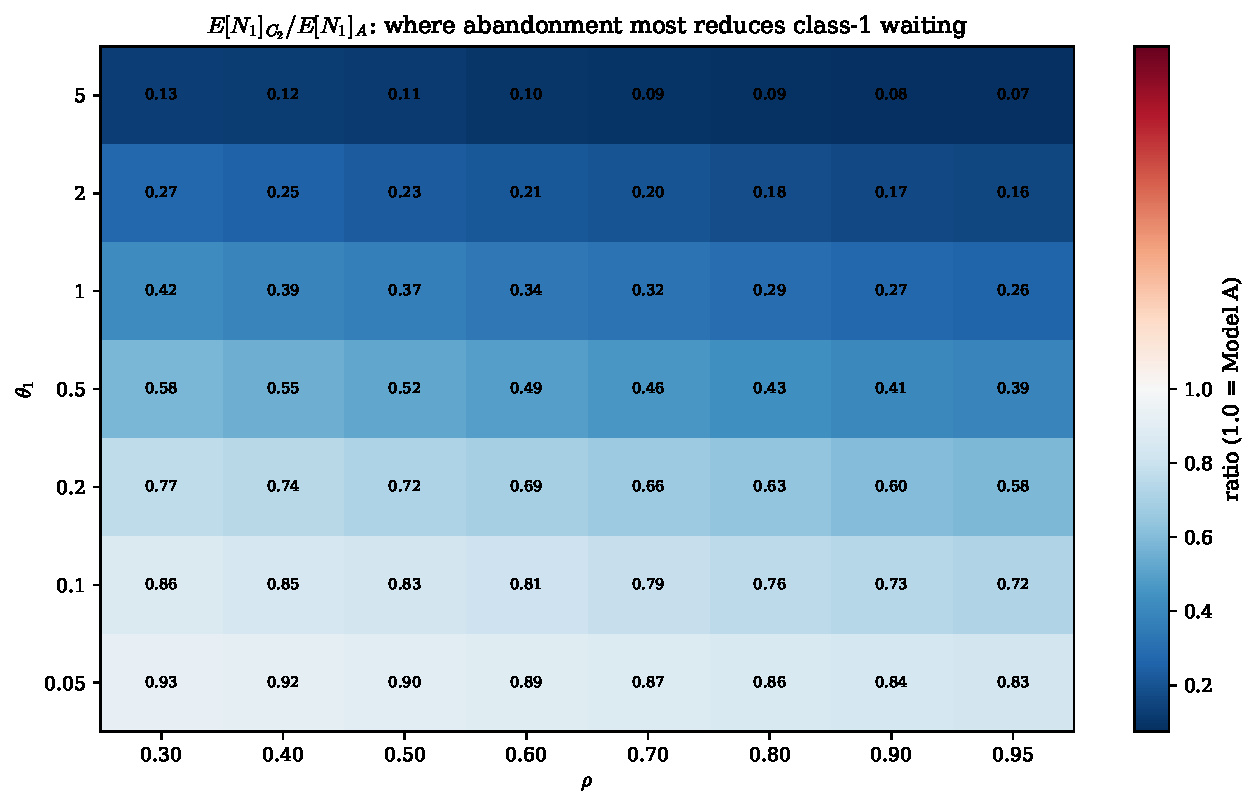
\includegraphics[width=0.85\textwidth]{figures/results/fig_C2_rho_theta_heatmap.pdf}
  \caption{Ratio $\mathbb{E}[N_1]_{C_2}/\mathbb{E}[N_1]_A$ over the $(\rho,\theta_1)$ plane;
  the diverging scale is centred at $1.0$ (the Model-$A$ value). \emph{Colour convention}
  (shared with the validity map, Figure~\ref{fig:val_ppgf}): \textcolor{green!60!black}{green}
  marks the favourable regime---ratio $<1$, where abandonment shortens the priority
  queue---and \textcolor{red}{red} the unfavourable regime, ratio $>1$; yellow is the
  break-even Model-$A$ value. Abandonment delivers its
  largest relative reduction in the priority queue at high load and high $\theta_1$
  (bottom-right region), exactly where the baseline backlog is most severe.}
  \label{fig:c2:heatmap}
\end{figure}

Read across the panel, the ratio varies far more strongly down the $\theta_1$ axis than along
the $\rho$ axis, so it is the \emph{valve strength}, not the offered load, that is the
first-order control on how much abandonment helps the priority class. Further $\theta_1$-sweeps
are deferred to Appendix~\ref{app:numerics:sweep}.

\end{document}
